\chapter{Stand der Technik}
\begin{onehalfspace}  
    \label{sec:theorie/standdertechnik}
        In diesem Kapitel wird der Stand der Technik näher beleuchtet. Der Fokus liegt dabei auf den Themen Daten, \ac{KI} und Bias. Zu Beginn wird auf basis der Literatur erläutert, was Daten sind, was Datenqualität bedeutet und worum es sich bei einem Bias handelt. Daraufhin wird näher auf \ac{KI}, das Teilgebiet \ac{ML} und die Ethik in der \ac{KI} eingegangen. Zuletzt werden die Themen in einen gemeinsamen Kontext gesetzt und der Einfluss eines Bias auf eine \ac{KI} betrachtet und Gegenmaßnahmen untersucht. 
    
    \section{Daten als wertschöpfende Ressource}
    \label{subsec:datenchapter}
    \subsection{Daten}
    \label{subsubsec:daten}
        Dass Daten eine wertvolle Ressource seien, meinte bereits 2006 der britische Mathematiker Clive Humby mit dem berühmten Zitat: \glqq{}Data is the new oil\grqq{}. Hiermit ist gemeint, dass Daten in ihre Rohform nicht sonderlich wertvoll sind, jedoch sobald man beginnt sie zu verarbeitet gewinnen sie an Wert. Denn lange Zeit waren Daten nur ein Nebenprodukt der Digitalisierung. Daten wurde gesammelt und gespeichert, aber nicht weiter verwendet. Mit dem technologischen Fortschritt im Bereich von Datenanalysen und mit aufkommen der \ac{KI} wurden Daten von Zeit zu Zeit immer wertvoller. So wurden neue Datengetriebene Geschäftsfeld eröffnet und ein Mehrwert aus Rohdaten geschaffen. Insbesondere das rasante Aufkommen des Internet of Things hat diese Entwicklung stark vorangetrieben. Seither steigt die Menge der jährlich gesammelten Daten exponentiell an.\cite{Otto2019}
        \\
        \begin{figure}[h]
            \centering
            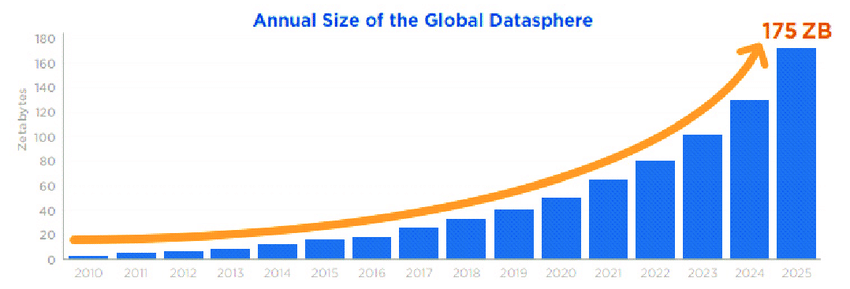
\includegraphics[width = 15.5cm]{Bilder/Annual_Data_Size.png}
            \caption{Weltweit jährlich anfallende Datenmenge \cite{Reinsel2018}}
            \label{fig:DataSize}
        \end{figure}
        \\
        Abbildung \ref{fig:DataSize} stammt aus dem Jahr 2018 und verdeutlicht, dass bereits damals erwartet wurde, dass bis im Jahr 2025 rund 175 Zetabyte Daten jährlich gesammelt werden. Im Vergleich dazu waren es 2018 gerade einmal 33 Zetabyte weltweit. \cite{Reinsel2018}
        \\
        Der Begriff Daten selbst wird im ISO2382-1 Standard wie folgt definiert: \glqq{}reinterpretierbare Darstellung von Informationen in einer formalisierten Weise, die für die Kommunikation, Interpretation oder Verarbeitung geeignet ist\grqq{}. \cite{ISO2382} Daraus lässt sich ableite, dass Daten Informationen der Vergangenheit repräsentieren und für zukünftige Verwendung die Informationen aus der Vergangenheit in einer einheitlichen Form repräsentieren. Damit ist jedoch nicht die einheitliche Form der Daten selbst gemeint. 
        \\
        Daten gibt es in unterschiedlichen Formen. Es wird zwischen strukturierten und unstrukturierten Daten unterschieden. Strukturierte Daten sind Datensätze bestehend aus einzelnen Variablen die eindeutige Größen Darstellen. Beispiel hierfür sind Sensordaten oder Unternehmenszahlen aus einem ERP System. Sie werden tabbelarisch gespeicher und können einfach weiter verarbeitet werden. Oftmals sind diese Daten heterogen, was bedeutet, dass sich die Variablen unterschieden und bspw. Spalte 1 vollkommen andere Daten behinhaltet als Splate 2. Ein Beispiel hierfür wären Sensoren für Luftfeuchtigkeit und Helligkeit in einem Büro. Als unstrukturierte Daten bezeichnet man Daten, die nicht in sinnvolle einheitliche Variablen unterteilt werden können. Zu dieser Art von Daten zählt man Bilder, Videos, Audio und Textdaten. Sie sind meist homogen, denn die Pixel in einem Bild nehmen zwar unterschiedliche RGB Werte an, jedoch repräsentieren sie alle einen Pixel. Dabei ist es egal ob es sich um Pixel 1 oder Pixel 42 handelt. \cite{Horn2022} Bei dieser unvorstellbar großen Datenmenge die jährlich generiert wird, wird davon ausgegangen, dass rund 80\% als unstrukturierte Daten vorliegen. \cite{Otto2019}
        \\
        In Rohform sind die Daten, wie eingangs erwähnt, nicht sonderlich von Wert. Mehrwert und Infromationen liefern sie erst, sobald man sie nutzt. Dabei ist es egal ob für Simulationen, Monitoring oder \ac{KI}. In der Vergangenheit sind Daten ein Nebenprodukt der Digitalisierung gewesen. Heute sind sie ein eigenes Geschäftsfeld und Enabler für viele bisher nicht möglich gewesenen Anwendungen. \cite{Otto2019} \cite{Gröger2021}

    \subsection{Datenqualität}
    \label{subsubsec:datenqualität}
        Im Zusammenhang mit Daten fällt immer häufiger auch der Begriff Daten Qualität. Hier trifft Quantität auf Qualität. Wie bereits erwähnt, ist die Menge an Daten die bereits zur Verfügung steht, rießig. Quantität ist daher nicht das Problem. Die Qualität der Daten hat hier jedoch sehr großen Einfluss. Nicht selten können Daten nicht verwendet werden, da die Qualität nicht ausreichend ist. Gerade für Analysen, Auswertungen und Vorhersagen, wie sie durch die \ac*{KI} getroffen werden sollen, benötigen eine hohe Datenqualität. 
        \\
        - 80 Prozent der Arbeit eines Data Scientist ist das Daten vorverarbeiten aufgrund schlechter Datenqualität
        - Data Quality Management
        - Data Qaulity Richtlinien und Anforderungen
        - Metadaten --> Das wissen über die Daten, was sollten die Daten repräsentieren und tun sie das auch

    \subsection{Bias}
    \label{subsubsec:Bias}
        -   Begriffserklärung: Data Bias vs Bias Verzerrung / Over-/Underfitting (zu viel/zu wenig lernen im ml)\\
        -   Arten von Bias: \\
            -   Bias durch Abwesenheit - Wenn eine Info fehlt, kann das zu Diskriminierung führen. \\
            -   Diskriminierung durch Menschen. \\
        Arten von Bias: Cognitive, Social, Perceptual und Motivational Bias \cite{Parkavi2018}


    \newpage
    \section{Künstliche Intelligenz}
    \label{subsec:KIandML}
    \subsection{Künstliche Intelligenz Allgemein}
    \label{subsubsec:KIAllgemein}
        - Was bildet KI alles ab <-- Grafik B. Otto?
        - KI als Geschäftsfeld 
        - KI und seine potentiale Ausleuchten 
        - Was ist alles KI
        - Wie definiert sich KI


    \subsection{Teilgebiet maschinelles Lernen}
    \label{subsubsec:teilgebietML}
        - Wie funktioniert ML --> Daten die gesammelt werden
        - Bewertete Daten aus der Vergangenheit --> Daten bewerter Jobs <-- Quelle
        - Welche Risiken - over under fitting etc.
        -   Superviced learning --> Data Bias\\
        -   Unsuperviced learning --> nicht zwingend Data Bias\\


    \subsection{Ethik in der künstlichen Intelligenz}
    \label{subsubsec:ethikinderKI}
        - Ethik spielt eine große Rolle in der Gesellschaft
        - EU Setzt sich mit Richtlinien auseinandern
        - Diskriminierung durch KI ist ein fatales Problem
        - Maschinen besitzen keine Moral und Ethisches werteverständnis


    \newpage
    \section{Bias im Zusammenhang mit \ac{KI}}
    \label{subsec:KIundbias}
    \subsection{Diskriminierung durch Bias in Daten}
    \label{subsubsec:diskriminierungdurchverzerrung}
        - Bias in Daten
        - Wie funktioniert Bias in Daten
        - Was ist die Problematik
        - Welche Auswirkungen hat es 
        - Realbeispiele <-- Bewerbungsverfahren

    \subsection{Gegenma{\ss}nahmen}
    \label{subsubsec:gegenmassnahmen}
        - Was kann man dagegen tun?
        - Gibt es möglichkeiten Trainingsdaten künstlich zu erzeugen und so eine neutrale betrachtung zu schaffen
        - Parameter entfernen als Lösung --> Die KI wird aber dadurch schlechter 
        - 

        Wenn der Parameter mit dem Bias entfernt wird, wird das Ergebnis erstmal schlechter. 
        
    \newpage
\end{onehalfspace}